\documentclass[]{article}
\usepackage{lmodern}
\usepackage{amssymb,amsmath}
\usepackage{ifxetex,ifluatex}
\usepackage{fixltx2e} % provides \textsubscript
\ifnum 0\ifxetex 1\fi\ifluatex 1\fi=0 % if pdftex
  \usepackage[T1]{fontenc}
  \usepackage[utf8]{inputenc}
\else % if luatex or xelatex
  \ifxetex
    \usepackage{mathspec}
  \else
    \usepackage{fontspec}
  \fi
  \defaultfontfeatures{Ligatures=TeX,Scale=MatchLowercase}
\fi
% use upquote if available, for straight quotes in verbatim environments
\IfFileExists{upquote.sty}{\usepackage{upquote}}{}
% use microtype if available
\IfFileExists{microtype.sty}{%
\usepackage{microtype}
\UseMicrotypeSet[protrusion]{basicmath} % disable protrusion for tt fonts
}{}
\usepackage[margin=1in]{geometry}
\usepackage{hyperref}
\hypersetup{unicode=true,
            pdftitle={CMPSC 250 Final Project: Final Report},
            pdfauthor={Xingbang Liu, Matt Jones, Travis Thomas},
            pdfborder={0 0 0},
            breaklinks=true}
\urlstyle{same}  % don't use monospace font for urls
\usepackage{longtable,booktabs}
\usepackage{graphicx,grffile}
\makeatletter
\def\maxwidth{\ifdim\Gin@nat@width>\linewidth\linewidth\else\Gin@nat@width\fi}
\def\maxheight{\ifdim\Gin@nat@height>\textheight\textheight\else\Gin@nat@height\fi}
\makeatother
% Scale images if necessary, so that they will not overflow the page
% margins by default, and it is still possible to overwrite the defaults
% using explicit options in \includegraphics[width, height, ...]{}
\setkeys{Gin}{width=\maxwidth,height=\maxheight,keepaspectratio}
\IfFileExists{parskip.sty}{%
\usepackage{parskip}
}{% else
\setlength{\parindent}{0pt}
\setlength{\parskip}{6pt plus 2pt minus 1pt}
}
\setlength{\emergencystretch}{3em}  % prevent overfull lines
\providecommand{\tightlist}{%
  \setlength{\itemsep}{0pt}\setlength{\parskip}{0pt}}
\setcounter{secnumdepth}{0}
% Redefines (sub)paragraphs to behave more like sections
\ifx\paragraph\undefined\else
\let\oldparagraph\paragraph
\renewcommand{\paragraph}[1]{\oldparagraph{#1}\mbox{}}
\fi
\ifx\subparagraph\undefined\else
\let\oldsubparagraph\subparagraph
\renewcommand{\subparagraph}[1]{\oldsubparagraph{#1}\mbox{}}
\fi

%%% Use protect on footnotes to avoid problems with footnotes in titles
\let\rmarkdownfootnote\footnote%
\def\footnote{\protect\rmarkdownfootnote}

%%% Change title format to be more compact
\usepackage{titling}

% Create subtitle command for use in maketitle
\newcommand{\subtitle}[1]{
  \posttitle{
    \begin{center}\large#1\end{center}
    }
}

\setlength{\droptitle}{-2em}
  \title{CMPSC 250 Final Project: Final Report}
  \pretitle{\vspace{\droptitle}\centering\huge}
  \posttitle{\par}
\subtitle{Instructor: Dr.~Mohan}
  \author{Xingbang Liu, Matt Jones, Travis Thomas}
  \preauthor{\centering\large\emph}
  \postauthor{\par}
  \predate{\centering\large\emph}
  \postdate{\par}
  \date{02 May 2018}


\begin{document}
\maketitle

\begin{center}\rule{0.5\linewidth}{\linethickness}\end{center}

\subsection{Motivation}\label{motivation}

Our team was inspired by existing music suggestion platforms (ie.
Spotify, Pandora, Apple Music, etc,) to mimic their systems and add our
own creative twist on current song suggesting algorithms. This includes
features similar to other platforms including: ``favorites'' or ``liked
music'', ``DailyMix'' and ``Recommended for You'', sorting features such
as ``by artist'' and ``by genre'', and a ``cloud database*" that would
hold the list of all possible songs that the user can choose from.

Our work also builds directly off the previous work submitted in this
course, as well as building off existing algorithms in the field. We
built directly off of the music-sorting lab we submitted earlier this
year, to sort the users liked songs. The creative twist we added to our
algorithm suggestion takes a look at how we listen to music from a
different angle. Because music provides a ``rhythm or beat'' to many of
the things we do (whether it's dancing, work, etc.), we decided to try
to rate a user based on the speed of the rhythm (also known as Tempo).

\paragraph{Why is it important}\label{why-is-it-important}

This work acts as valuable research to anyone in the music industry.
Specifically, anyone who is looking at new ways to incorporate aspects
of songs into a user-song-suggestion platform. While current music
platforms are doing a good job of suggesting songs (usually based off
other real peoples songs), there's still songs that users find
out-of-the-blue on their own that they really enjoy. Exploring new ways
to relate aspects of songs to the user can only help find these outlying
songs, and suggest them to the user.

\paragraph{How is it useful}\label{how-is-it-useful}

Millions of people use music everyday. Whether it's to wake up to their
favorite song in the morning, make their commute to their job better, or
provide some-type of rhythm to everyday tasks, music makes our lives
better! So, a tool which helps you find music you like, and save music
you like would undoubtedly be useful to a lot of people.

\subsection{Background for problem}\label{background-for-problem}

There are many algorithms to find similar songs. Here are two examples
of the Collaborative ???ltering:

\paragraph{Memory-based}\label{memory-based}

Generaly, user would be grouped in this algorithm. In this method, the
algorithm will first track down people who have similar activities, then
recommend songs to each other by their playlists. For example, action
score could be assigned as:

\begin{longtable}[]{@{}ccccccc@{}}
\toprule
Repeat song & Share & Like & Play & Played completely & Skip &
Dislike\tabularnewline
\midrule
\endhead
5 & 4 & 3 & 2 & 1 & -1 & -5\tabularnewline
\bottomrule
\end{longtable}

Then, a persons preference would be a N-Dimensional vector. Here N is
the number of songs by default. By using the cosine of the vector angle,
which is generated by two vector, we can know how similar two users can
be. The cosine of 0 degree, which means two people are exactly the same,
is 1. The cosine of 180 degree, which means two people have the opposite
preference, is -1. The equation is:

Assume we have vector \(\vec a\) and \(\vec b\),

\[cos(A) = \frac{\vec a \cdot \vec b}{|\vec a| \times |\vec b|}\]

This prediction method is very accurate, but there are too many
calculations and it is not accurate for a new user.

\paragraph{Model-based}\label{model-based}

As for the second method, the algorithm will analyze the playlist of a
person, then do recommendations. Models such as the latent factor are
used in this method. In latent factor model, user's like list will be
analyzed by dividing into different tag factors, for example, classic
and indie. By signing scores for different factor, we can have a matrix
which can divided into two different matrix:

\[R = QP^T\] \[R_{user,song}= Q_{user,factor} P^T_{factor,song}\] \[=
\begin{pmatrix}
  q_{user_{1},factor_{1}} & q_{user_{1},factor_{2}} & \cdots & q_{user_{1},factor_{n}} \\
  q_{user_{2},factor_{1}} & q_{user_{2},factor_{2}} & \cdots & q_{user_{2},factor_{n}} \\
  \vdots  & \vdots  & \ddots & \vdots \\
  q_{user_{n},factor_{1}} & q_{user_{n},factor_{2}} & \cdots & q_{user_{n},factor_{n}}
  \end{pmatrix}\] \[
  \begin{pmatrix}
  p_{factor_{1},song_{1}} & p_{factor_{1},song_{2}} & \cdots & p_{factor_{1},song_{n}} \\
  p_{factor_{2},song_{1}} & p_{factor_{2},song_{2}} & \cdots & p_{factor_{2},song_{n}} \\
  \vdots  & \vdots  & \ddots & \vdots \\
  p_{factor_{n},song_{1}} & p_{factor_{n},song_{2}} & \cdots & p_{factor_{n},song_{n}}
  \end{pmatrix}^T\]

From the matrix R, we can get estimated score. After that, we can ignore
the song which the user already listened, and recommend him the song he
has not listened.

Of course, in the real world, if we implement algorithm based on song,
the second dimension factor will rapidly increase. Plus there will be
too many songs. Therefore, it will be more efficient if we calculate
based on tags of the song. For example, for ``The Sound of Silence'' by
Simon \& Garfunel, tags can be Folk Rock, 60s, and Movie Track. Due to
the time we have is limited, we would not build tags databases,
therefore we would analyze by songs.

In the real situation, based on different requirements, we can pick one
of them or use them together. It is also an option to mix these two
algorithms and form a new hybrid algorithm when there are not enough
songs in a playlist.

\paragraph{How could it be improved}\label{how-could-it-be-improved}

These algorithms are not perfect, they could be limited when there are
not enough users. For example, if a start up music service company wants
to suggest songs to user, they have to use an algorithm which works when
there are not enough users and user action data. In this situation, it
would be better if the company could depend on the music only, for
example, music metadata, rather than depend on user data. In our
algorithm, we hard coded melody scores, From 1 to 10, the faster the
higher, for each songs. This score simulated music classification data.
By getting a mean score from user liked list, we can find more songs by
their mean score. This method is more like a weaker version of the
combination of nature language processing and raw audio analyze. In
nature language processing, the program would analyze the lyrics, then
get the emotion data. In raw audio analyze, the program would analyze
the audio frames, and finally get an score for audio characteristic.

\subsection{Program and Algorithm
Description}\label{program-and-algorithm-description}

\paragraph{Pseudocode}\label{pseudocode}

\texttt{For\ each\ liked\ song:} \texttt{append\ to\ likedlist;}
\texttt{mean\ =\ (sum\ of\ melodies)/likedListLength;}
\texttt{for\ exploreSong{[}\textquotesingle{}melody\textquotesingle{}{]}\ ==\ mean:}
\texttt{return\ song;}

This is a very basic description of the algorithm but it explains the
though process behind the algorithm used to return songs. Essentially,
we ask the user pick songs that they like. This will add those liked
songs to the liked list. Using, the songs from the liked list, we find
the mean of the melodies within the liked list. This mean is then used
to search the main music database and return a set of songs that match
the mean melody score of the liked list. The melody score is just one
way we can return a set of recommended songs, there are other variables
that can be and will be included in the future. The inclusion of these
variables will not only give us a more desirable list of recommended
songs for user but will also allow for options when returning a set of
songs. For example, if a user wants a playlist to workout to, we may
want to return songs with high melody scores that are more upbeat.

\paragraph{Diagram}\label{diagram}

\textbf{Figure 1} is a basic outline of the interaction between classes
in our program. The \texttt{music.csv} file is fed into
\texttt{explore.java}, returning random songs with its explore function
and also sends the liked songs to \texttt{liked.csv} with its add
function. The liked songs are used by \texttt{DailySelection.java} and
\texttt{Like.java}. DailySelection uses the algorithm discussed in the
pseudocode to return songs that match the mean melody rating of the
songs found in the liked list. The Like class sorts the liked list by
either song, genre, artist, or year. \texttt{Like.java} calls
\texttt{SortInt} to sort the year and \texttt{SortString.java} to sort
the other categories. \texttt{MusicSug.java} is the main method and
gives the user a command-line interface to interact with music
recommender system, calling the functions mentioned above.

\paragraph{Time Complexities}\label{time-complexities}

\textbf{Figure2} Represents the time complexities of the Bubble sort and
Exchange sort after four runs. \texttt{SortInt.java} utilizes the bubble
sort method to sort the year songs within the liked list.
\texttt{SortString.java} utilizes exchange sort to sort each of the
other categories. We found a worst-case time complexity of
O(n\textsuperscript{2}) for both sorting algorithms. We decided to used
these algorithms because we do not anticipate large scale growth in our
liked list in its current state. That is the program only accounts for a
single user and the user will not produce enough songs on the liked list
to mandate a different algorithm.

\subsection{Conclusion}\label{conclusion}

\paragraph{Results}\label{results}

While analyzing our results, note that our program doesn't take into
account things like artist, genre, instruments used, etc. when
suggesting songs. However, the program does take a unique approach to
song suggesting, and runs without any bugs (caused by the user and/or
built into our system).

\textbf{Figure 3} shows the Main Menu of our program. It offers four
options: Like (prints liked songs), Explore (Finds and adds new songs to
the users liked songs), Daily Selection (Makes a playlist similar to the
songs in the users liked-list), Quit (Exits the program)

\textbf{Figure 4} shows the first feature: Print Liked Songs \& Sort
them.

\textbf{Figure 5} shows the second feature: Finds 5 songs for the user,
and the user picks a song (in this case, song 3) to add to their liked
songs. Then \textbf{figure 6} shows the updated liked songs with new
addition from feature \#2.

\textbf{Figure 7} shows the third feature: Gives you two song selections
similar to your liked list tempo, and then the user adds these songs to
their liked songs.

\textbf{Figure 8} shows updated liked songs with new addition from
feature \#3.

\textbf{Figure 9} shows the fourth feature: Quit/exits the program.

\paragraph{Takeaways}\label{takeaways}

There are a few notable takeaways from researching and implementing our
final project. First, collaborative filtering algorithms are complex and
take into account many, many variables. There are many components that
make up a song, thus creating accurate predictions requires a lot of
data. Second, collaborative is difficult to implement if multiple users
are not involved. Our program only accounts for a single user and single
liked list. An optimal implementation would call for multiple user's
liked lists to be compared across the program, to find similar user
interests so we can recommend songs based off of similar user's
playlists and interests. Overall, are program is a solid first-step in
implementing a music recommender that is capable of taking in unique
parameters, such as melody score, to recommend songs to users.

\paragraph{Challenges}\label{challenges}

Their were a few obvious problems that our group encountered that was to
be expected. Because our program has many different working parts, we
had to split it up and then either comment the code in a way so that our
other group members could explain it. Alternatively to commenting every
bit of code, we also met many times to try to explain our code to the
rest of the group. The biggest challenge our group had was working with
the ``cloud music list'' (aka our Music.csv) and figuring out how to
edit this list without messing us the csv file and the rest of our
program. Our solution was to make a ``working csv file'' (Test.csv) that
was the file we actually made edits to, while the ``cloud file''
(Music.csv) was left alone so that the edits didn't cause any problems
with the rest of the program.

\subsubsection{Rewards}\label{rewards}

The process of this project as been rewarding at every step. The
research that went into the project to learn about collaborative
filtering and common algorithms used to recommend songs was interesting
as we all frequently use these music apps. So, learning how these apps
recommend daily playlists and songs that we may like is intriguing.
Implementation was rewarding in its challenges. Every obstacle overcame
was its own reward. We have newfound respect for programmers that are
responsible for implementing and maintaining these algorithms because we
know the amount of data and variables that goes into proper
implementation.

\subsection{Index}\label{index}

\begin{figure}
\centering
\includegraphics{../images/diagram.PNG}
\caption{diagram}
\end{figure}

\begin{figure}
\centering
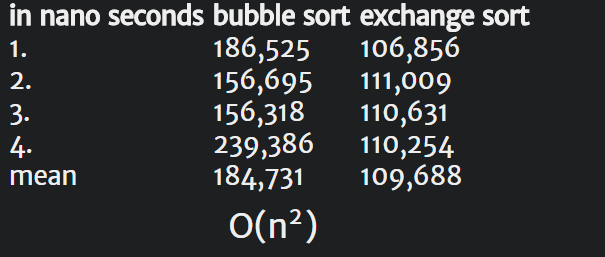
\includegraphics{../images/TimeComplex.PNG}
\caption{Time Complexities}
\end{figure}

\begin{figure}
\centering
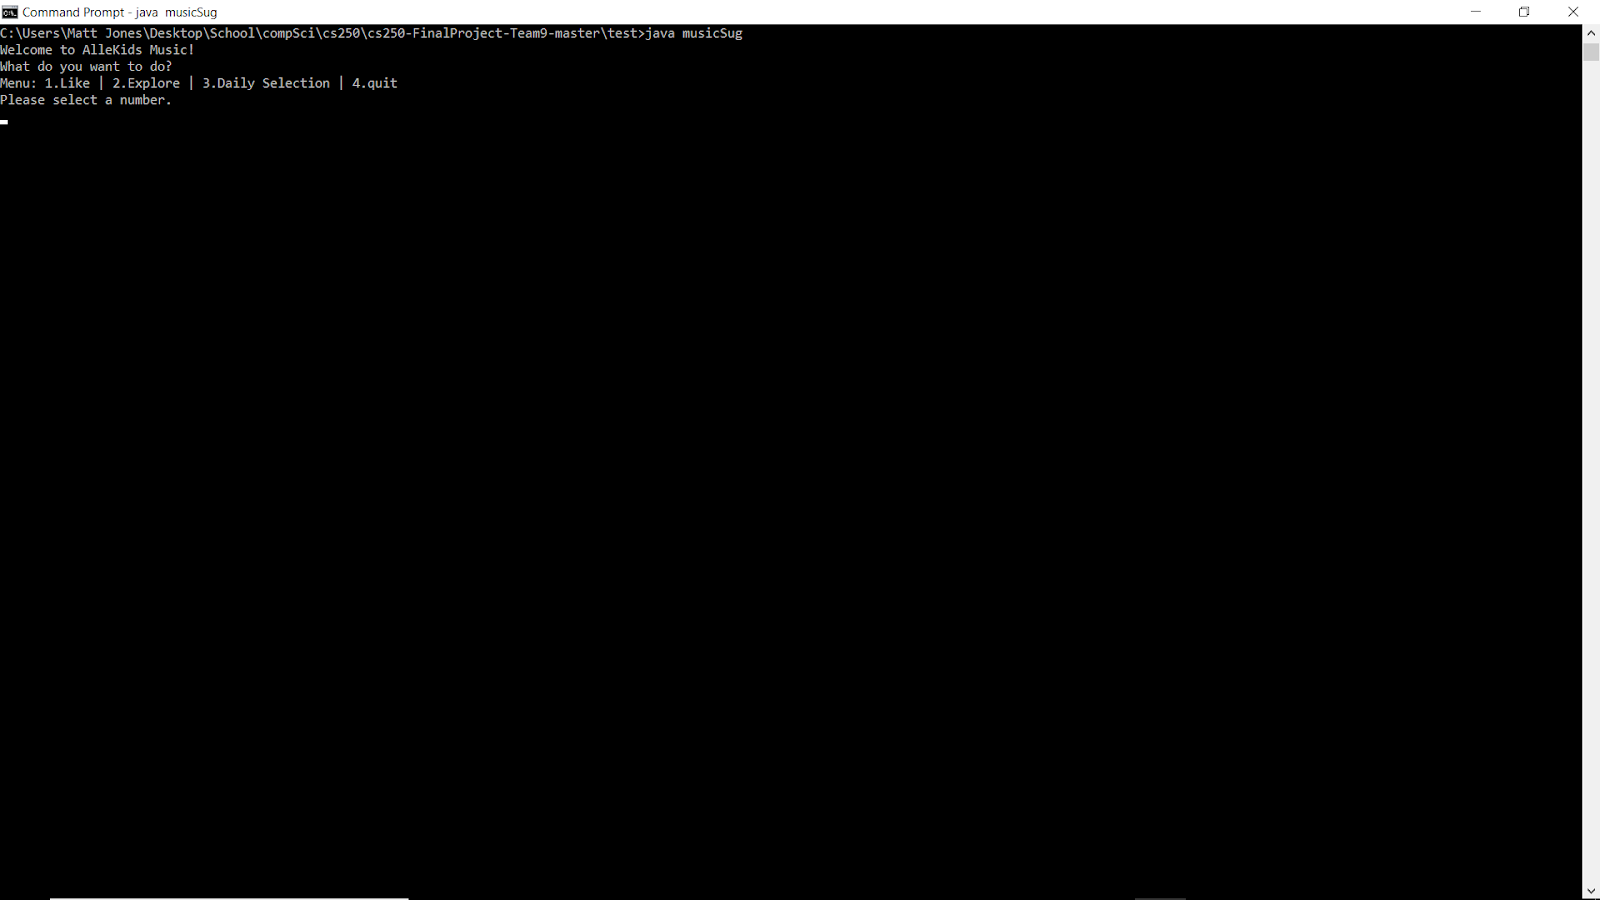
\includegraphics{../images/menu.png}
\caption{menu}
\end{figure}

\begin{figure}
\centering
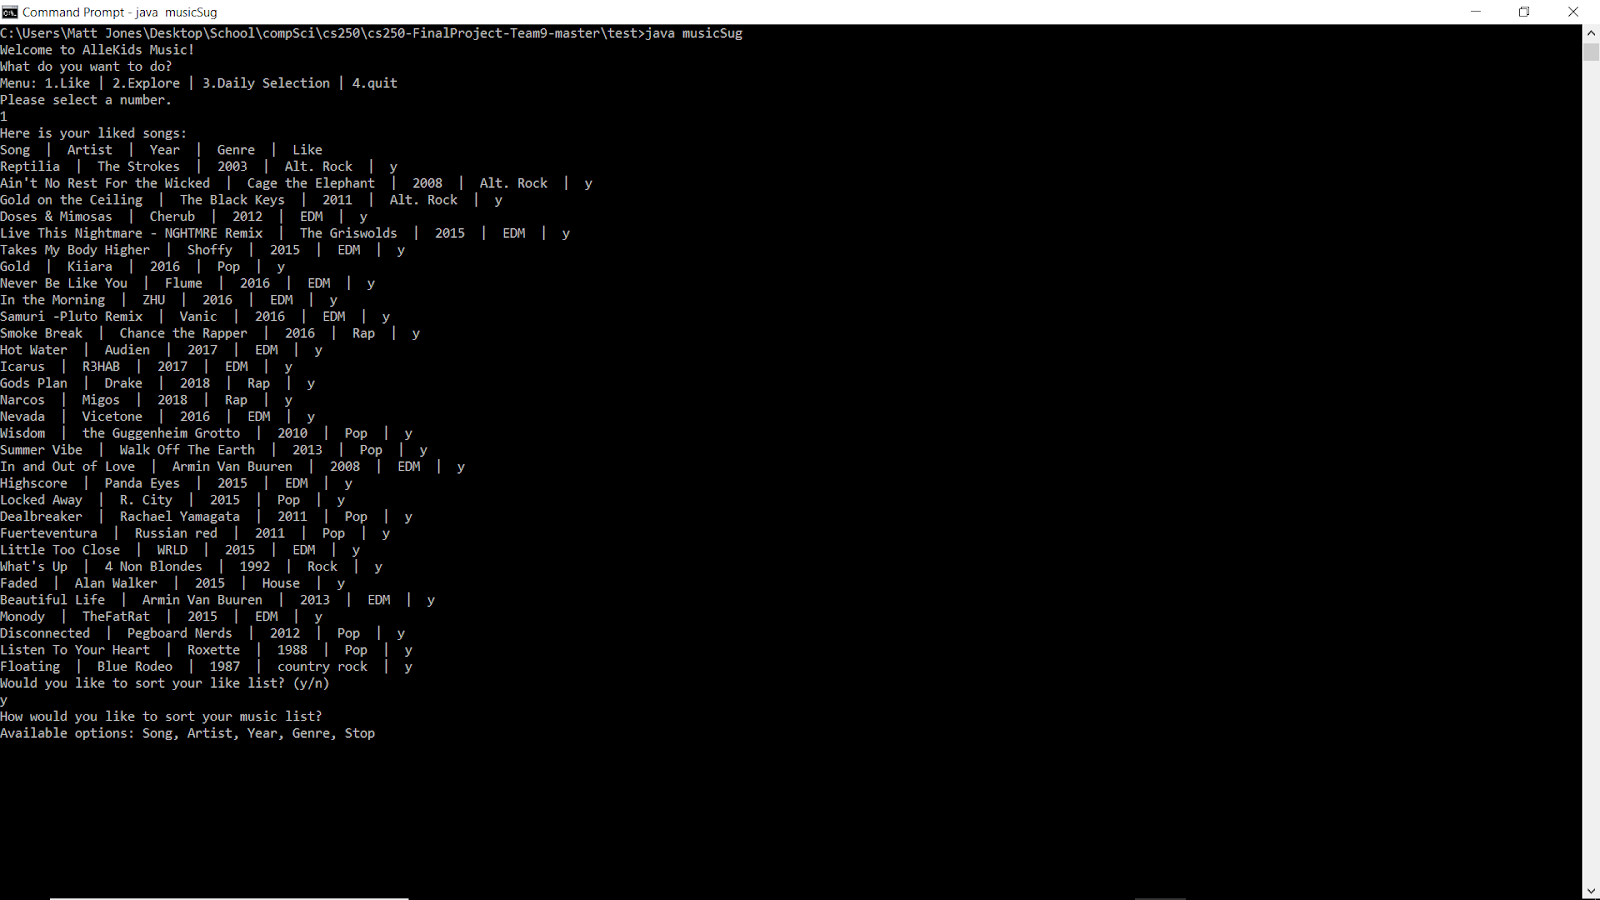
\includegraphics{../images/likeList.PNG}
\caption{print Liked Songs \& Sort them}
\end{figure}

\begin{figure}
\centering
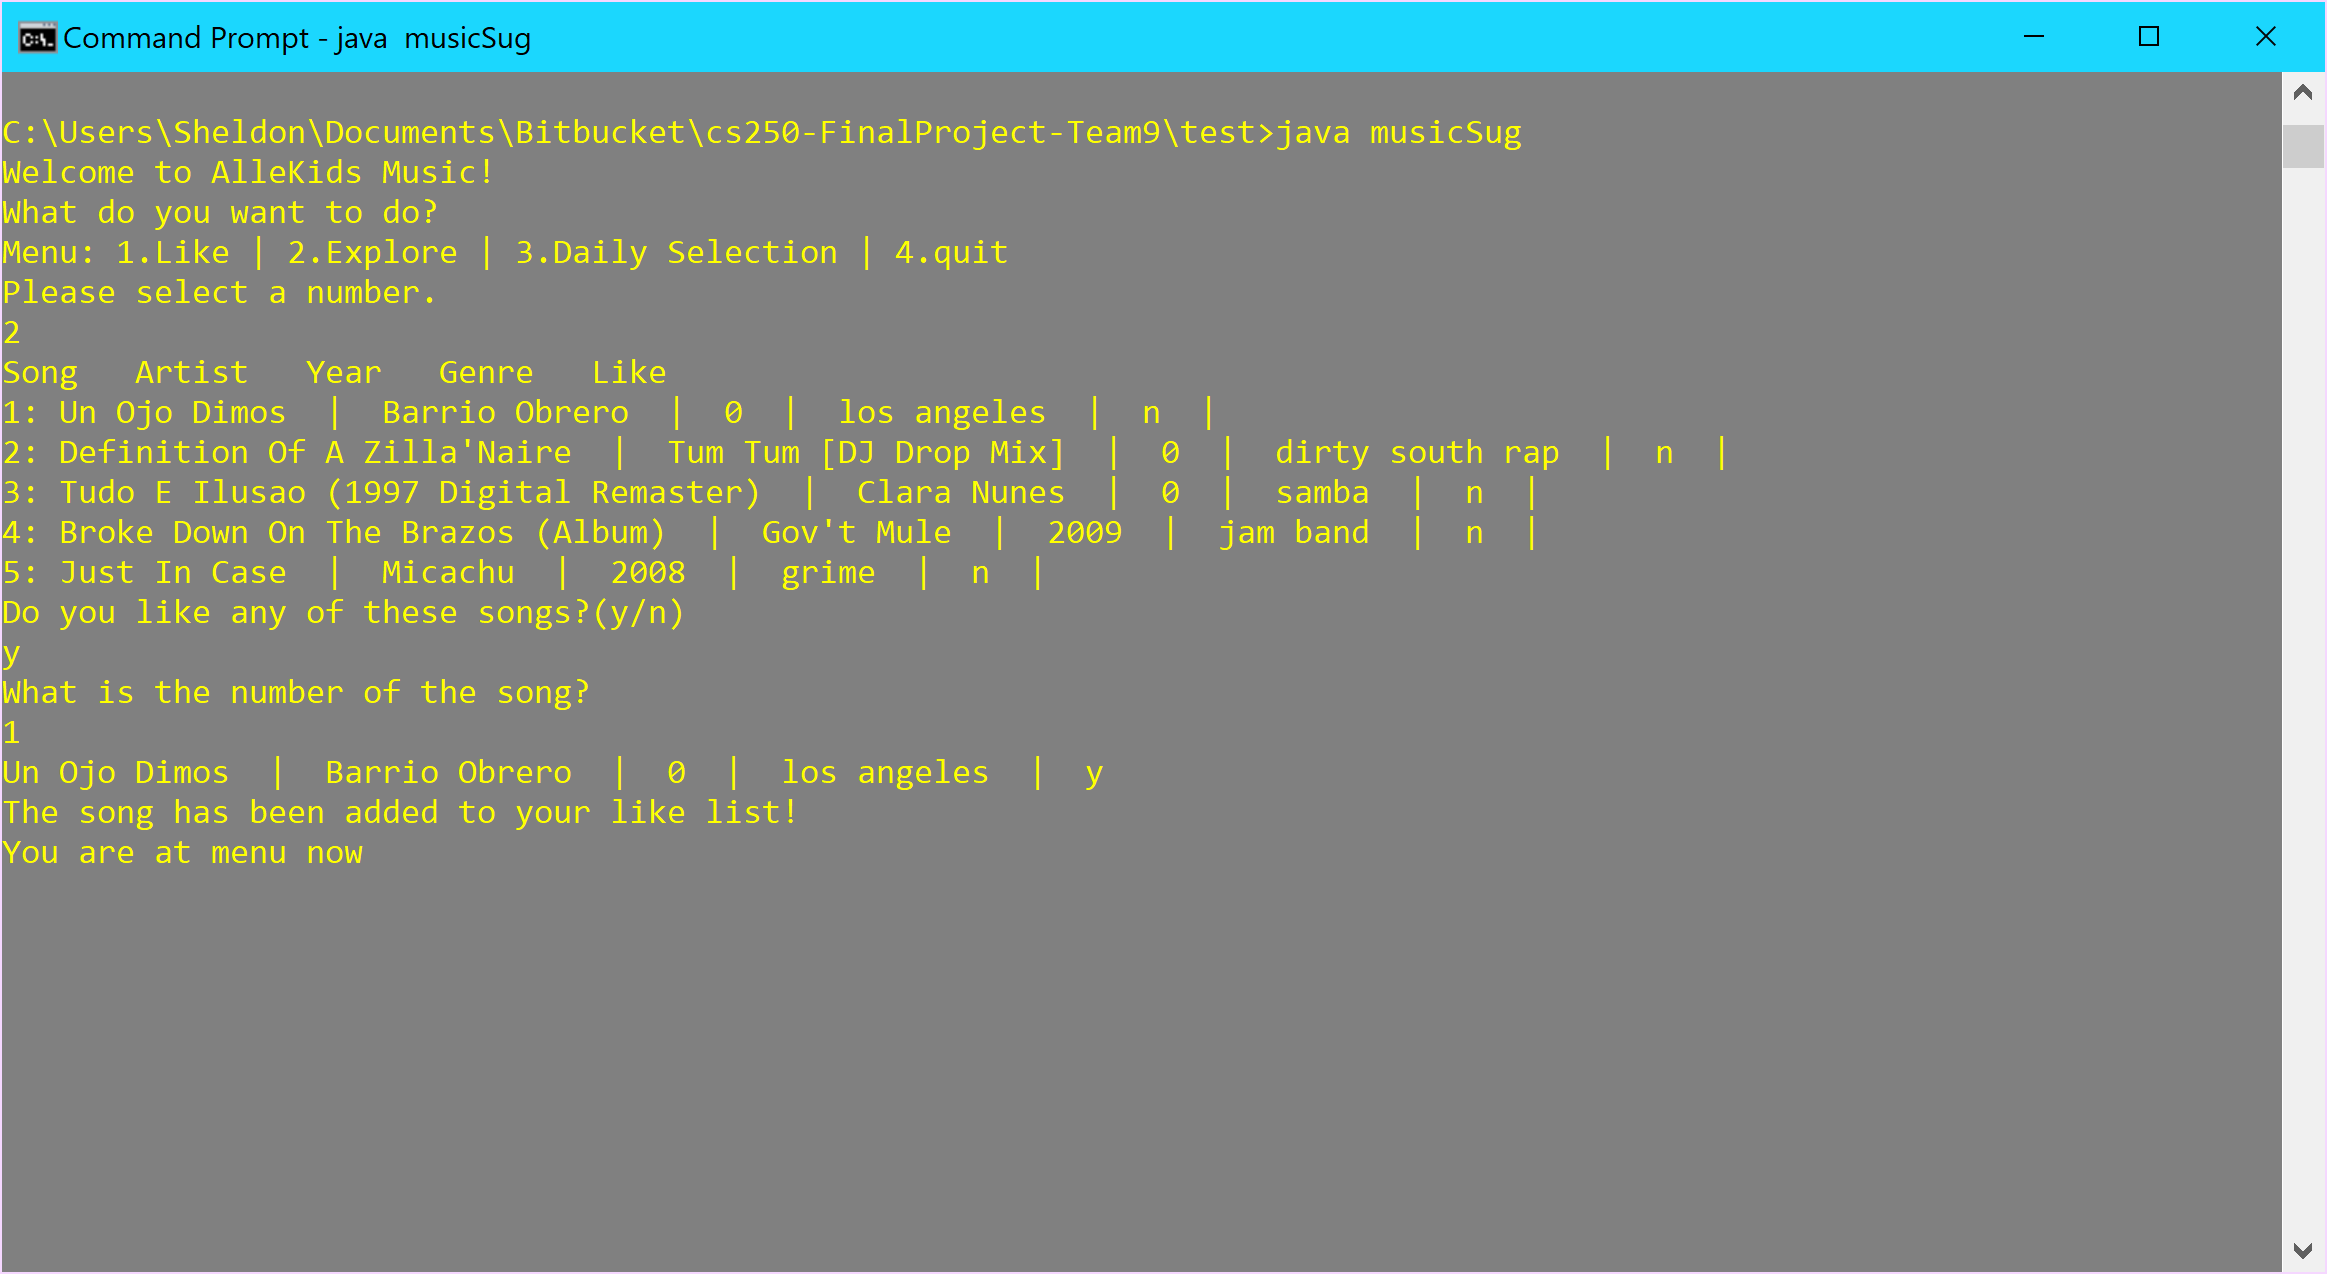
\includegraphics{../images/explore.PNG}
\caption{explore}
\end{figure}

\begin{figure}
\centering
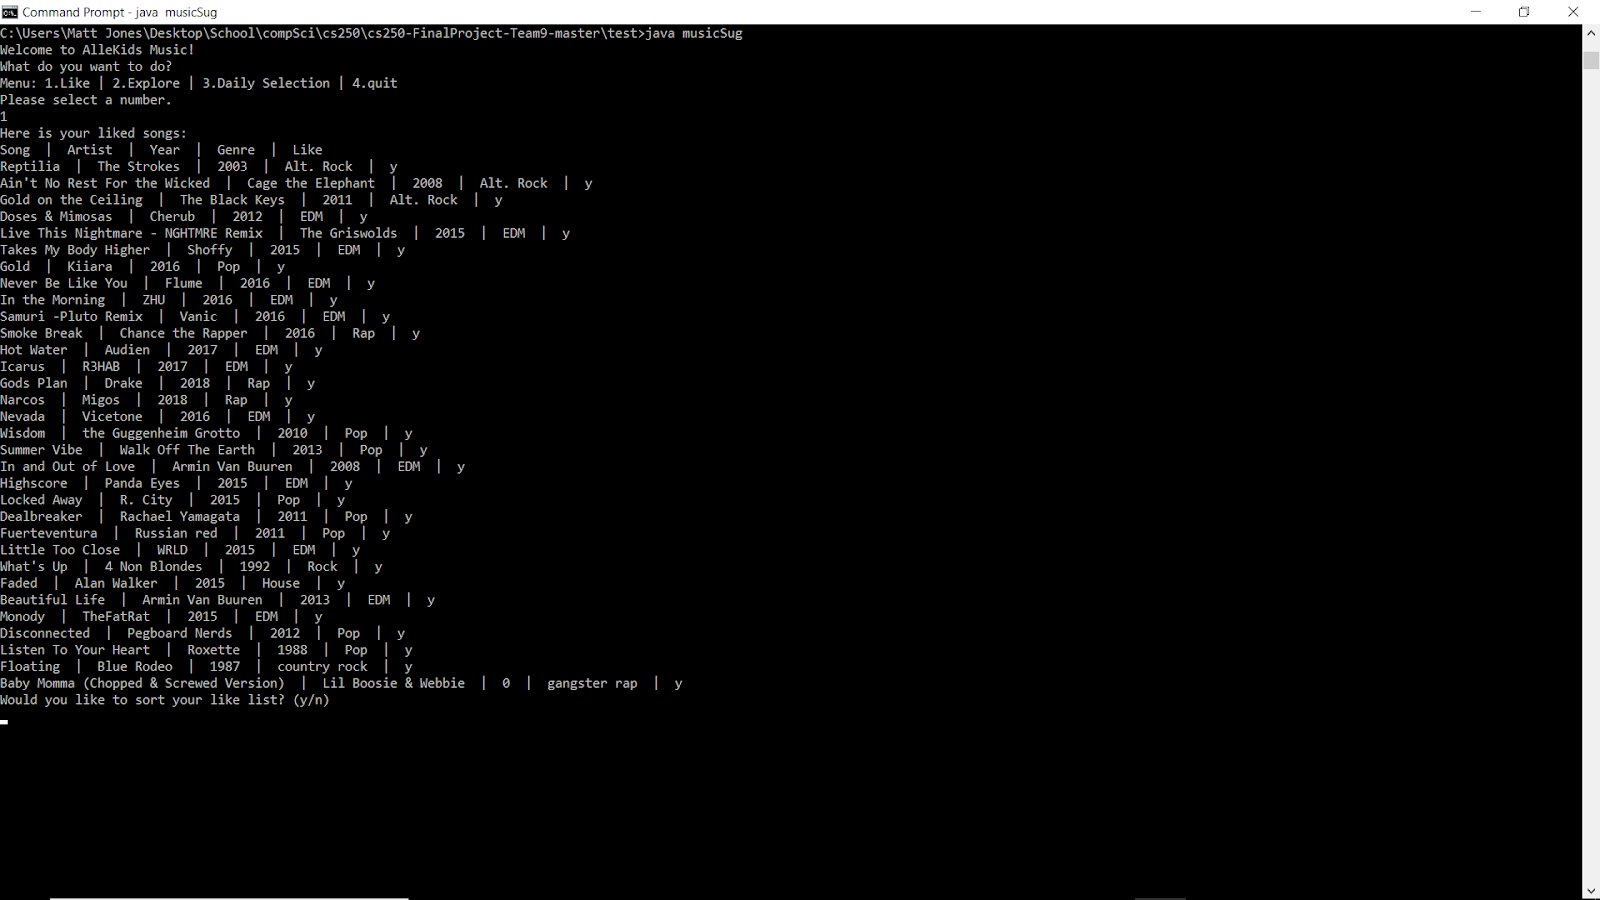
\includegraphics{../images/updated.png}
\caption{updated liked songs}
\end{figure}

\begin{figure}
\centering
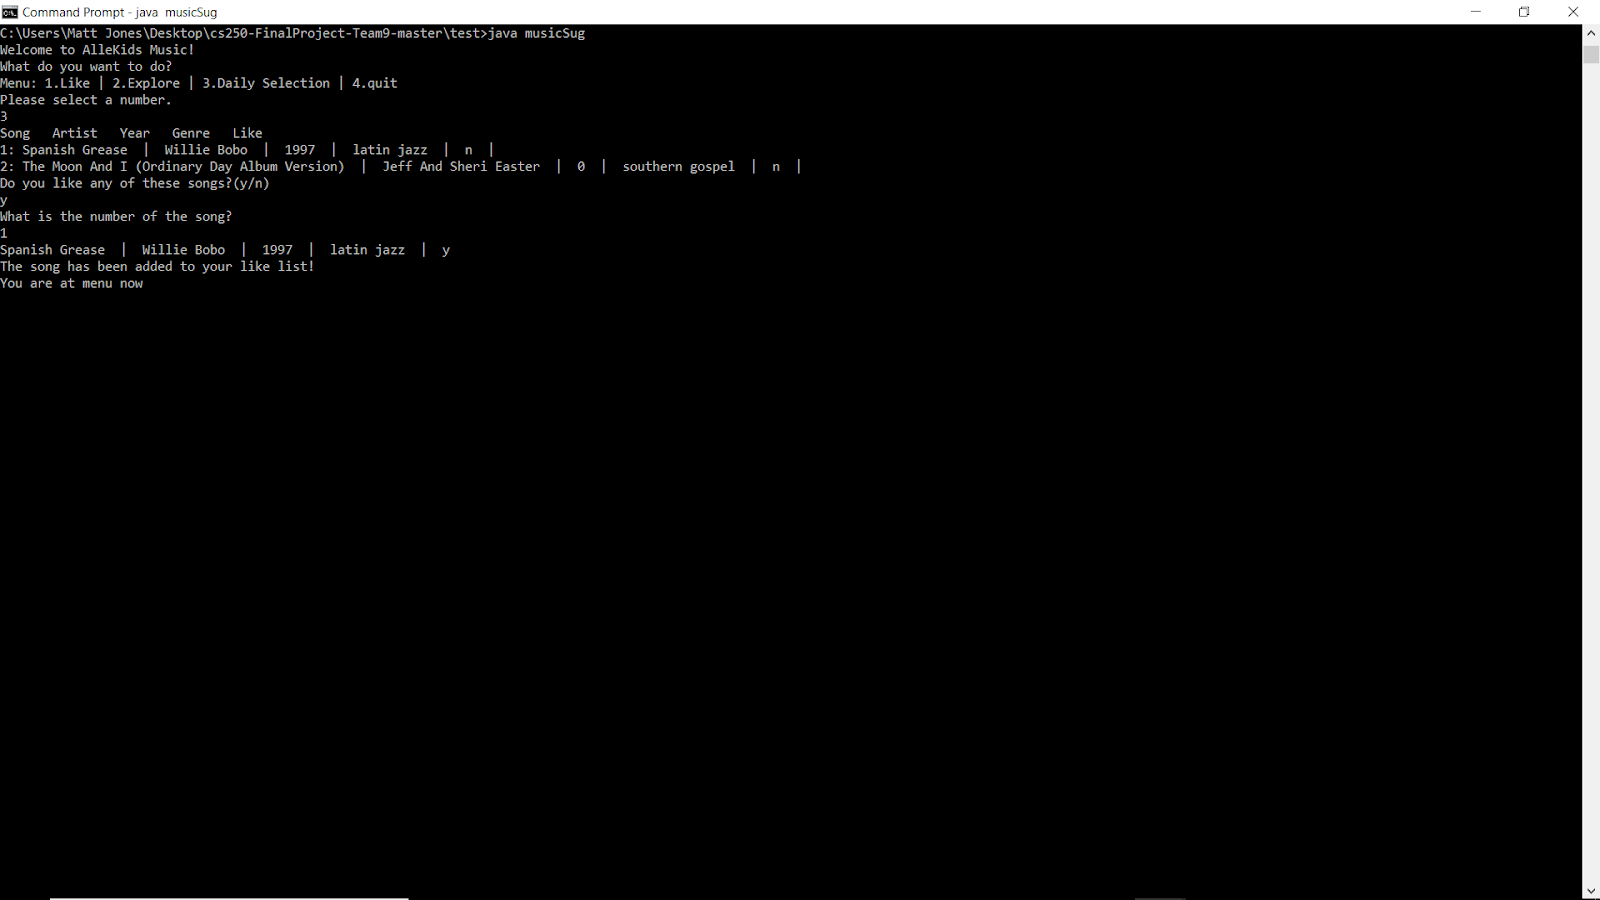
\includegraphics{../images/suggestion.PNG}
\caption{suggestion}
\end{figure}

\begin{figure}
\centering
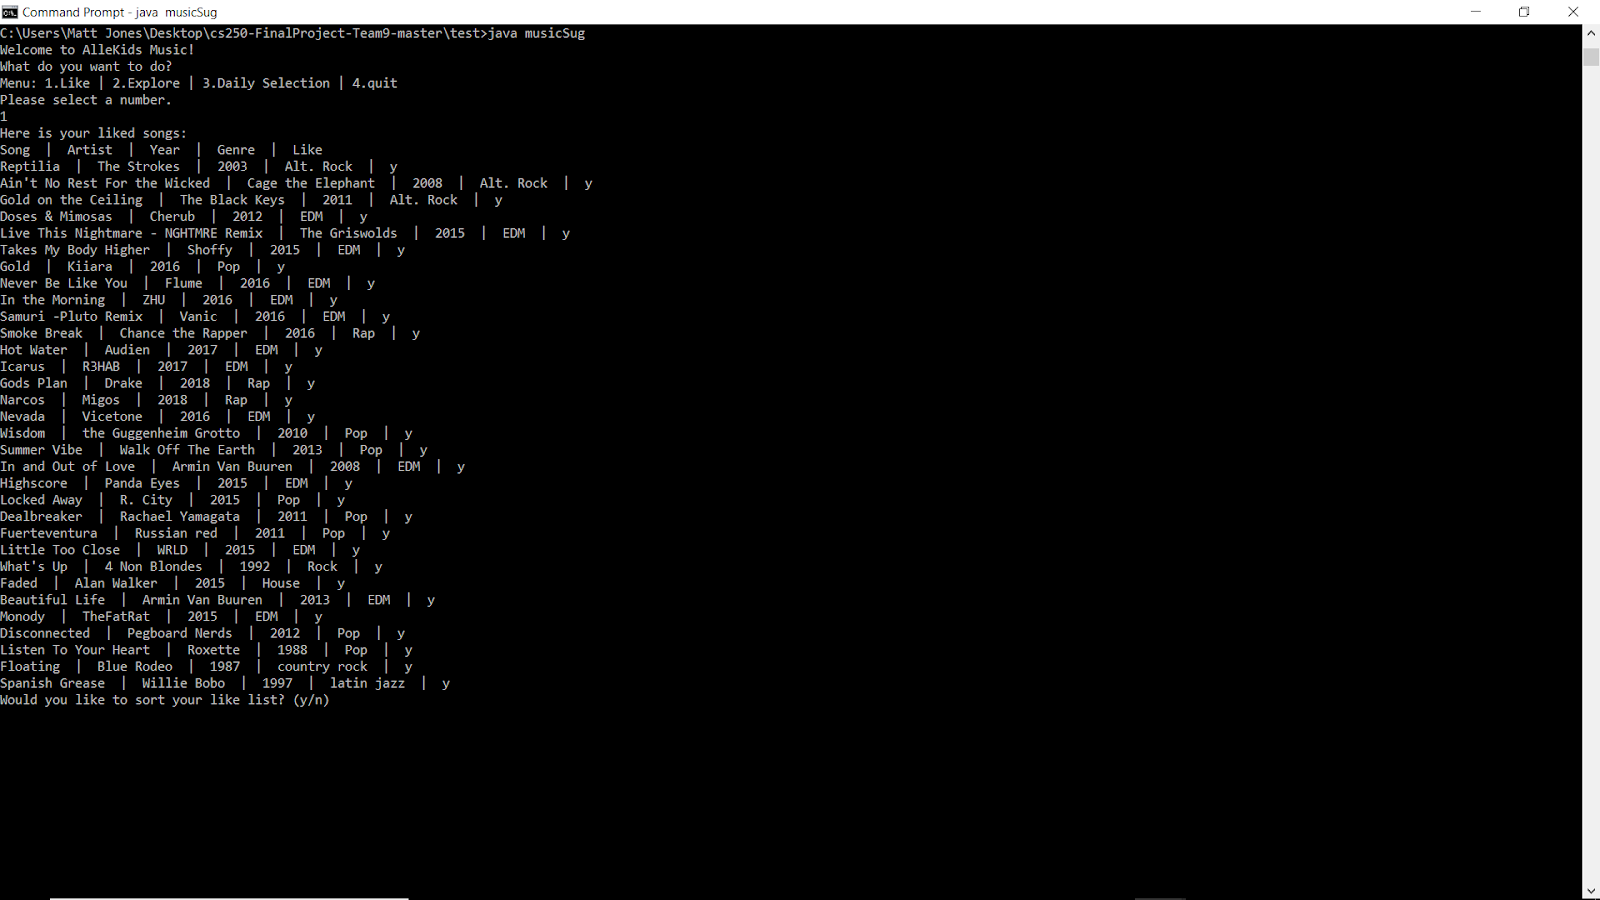
\includegraphics{../images/new.png}
\caption{updated liked songs}
\end{figure}

\begin{figure}
\centering
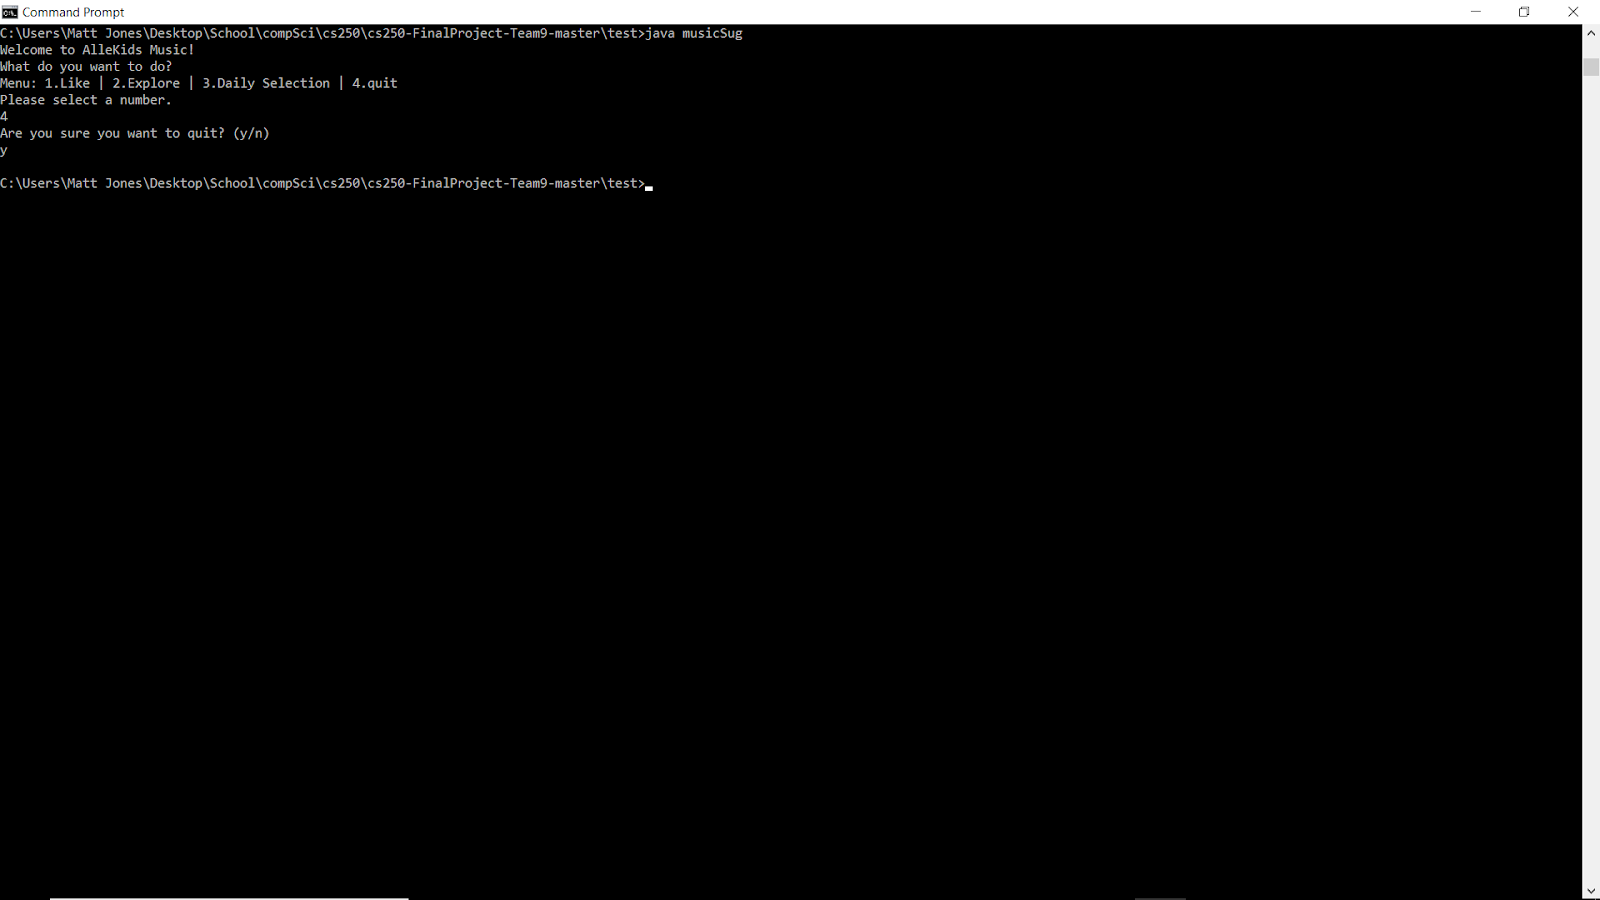
\includegraphics{../images/quit.png}
\caption{Quit/exits}
\end{figure}


\end{document}
